%; whizzy document
% latex beamer presentation.
% platex, latex-beamer でコンパイルすることを想定。 

%     Tokyo Debian Meeting resources
%     Copyright (C) 2006 Junichi Uekawa

%     This program is free software; you can redistribute it and/or modify
%     it under the terms of the GNU General Public License as published by
%     the Free Software Foundation; either version 2 of the License, or
%     (at your option) any later version.

%     This program is distributed in the hope that it will be useful,
%     but WITHOUT ANY WARRANTY; without even the implied warranty of
%     MERCHANTABILITY or FITNESS FOR A PARTICULAR PURPOSE.  See the
%     GNU General Public License for more details.

%     You should have received a copy of the GNU General Public License
%     along with this program; if not, write to the Free Software
%     Foundation, Inc., 51 Franklin St, Fifth Floor, Boston, MA  02110-1301 USA

% 実行順番
% sudo  ~/bin/usb-macbook-ir.c &
% real presentation (shell-command (concat "DISPLAY=:0.1 xpdf -fullscreen " (replace-regexp-in-string "tex$" "pdf"(buffer-file-name)) "&"))
% DISPLAY=:0.1 xpdf -fullscreen 

\documentclass[cjk,dvipdfmx]{beamer}
\usetheme{Warsaw}
%  preview (shell-command (concat "xpdf " (replace-regexp-in-string "tex$" "pdf"(buffer-file-name)) "&"))
%  presentation (shell-command (concat "xpdf -fullscreen " (replace-regexp-in-string "tex$" "pdf"(buffer-file-name)) "&"))

%http://www.naney.org/diki/dk/hyperref.html
%日本語EUC系環境の時
\AtBeginDvi{\special{pdf:tounicode EUC-UCS2}}
%シフトJIS系環境の時
%\AtBeginDvi{\special{pdf:tounicode 90ms-RKSJ-UCS2}}

\title{東京エリア Debian 勉強会}
\subtitle{資料}
\author{上川 純一 dancer@debian.org\\IRC nick: dancerj}
\date{2006年11月19日}
\logo{
\includegraphics[width=8cm]{image200607/openlogo-light.eps}}

% 三択問題用
\newcounter{santakucounter}
\newcommand{\santaku}[5]{%
\addtocounter{santakucounter}{1}
\frame{\frametitle{問題\arabic{santakucounter}. #1}
%問題\arabic{santakucounter}. #1
\begin{minipage}[t]{0.7\hsize}
 \begin{itemize}
 \item  A #2\\
 \item  B #3\\
 \item  C #4\\
 \end{itemize}
\end{minipage}
}
\frame{\frametitle{問題\arabic{santakucounter}. #1}
%問題\arabic{santakucounter}. #1
\begin{minipage}[t]{0.7\hsize}
\begin{itemize}
\item  A #2\\
\item  B #3\\
\item  C #4\\
\end{itemize}
\end{minipage}
\begin{minipage}[t]{0.2\hsize}
答えは:


\vspace{1cm}

{\huge \hspace{1cm}#5}
\end{minipage}}
}


\begin{document}
\frame{\titlepage{}}

\section{Intro}

\begin{frame}
 \frametitle{本日のagenda}
\begin{minipage}[t]{0.35\hsize}
  \begin{itemize}
   \item 今日の講師
   \item 上川\\
	 Debian JP 会長
   \item 岩松\\
	 Debian JP 副会長
 \end{itemize}
\end{minipage} 
\begin{minipage}[t]{0.6\hsize}
 \begin{itemize}
  \item 14:00-14:20 最近の Debian 勉強会の紹介
  \item 14:20-15:00 事前課題紹介
  \item 15:00-15:10 sid を日常環境として使うための注意, 上川
  \item 15:10-15:20 bugreport 論, 上川
  \item 15:30-16:00 パッケージングについて, 岩松
  \item 16:00-16:40 質問コーナー, 各位
  \item 17:00-18:00 京橋に移動
  \item 18:00-20:00 宴会
 \end{itemize}
\end{minipage}
\end{frame}

\begin{frame}
 \frametitle{KOF Debian BOF のアジェンダ}
\begin{minipage}[t]{0.4\hsize}
  \begin{itemize}
  \item 講師
	\begin{itemize} 
	 \item 上川\\
	       Debian JP 会長
	 \item 岩松\\
	       Debian JP 副会長
	 \item やまね\\
	       po-debconf翻訳職人
	\end{itemize}
 \end{itemize}
\end{minipage} 
\begin{minipage}[t]{0.4\hsize}
 \begin{itemize}
  \item Debian 紹介
  \item Debian JP 紹介
  \item エッチについて
  \item Debconf in Japan 進捗報告
 \end{itemize}
\end{minipage}
\end{frame}

\begin{frame}
 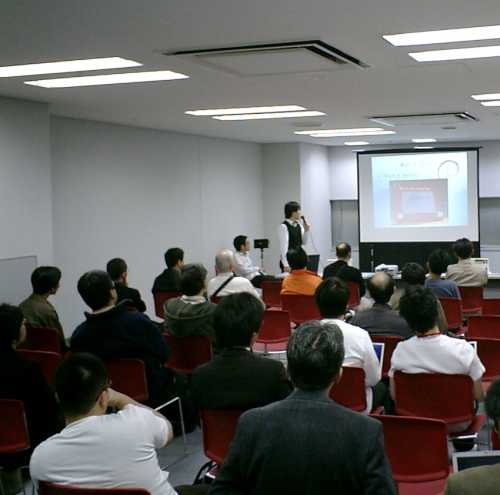
\includegraphics[width=0.8\hsize]{image200611/meeting.jpg}
\end{frame}


\begin{frame}
 \frametitle{10月のDebian勉強会のagenda}
\begin{minipage}[t]{0.4\hsize}
  \begin{itemize}
  \item 注意事項
	\begin{itemize}
	 \item 飲食禁止
	 \item 政治/宗教/営利活動禁止
	\end{itemize}
  \item 最近事情
  \item 事前課題紹介
  \item quiz
 \end{itemize}
\end{minipage} 
\begin{minipage}[t]{0.4\hsize}
\begin{itemize}
  \item スペイン参加報告
  \item flash ねた
  \item apt チューニングねた
 \end{itemize}
\end{minipage}
\end{frame}


\section{Debian Projectとは}
\begin{frame}{Debian Project}
 \begin{itemize}%[<+->]
  \item 1つの社会契約、ポリシー
  \item 10のアーキテクチャ
  \item 100のメーリングリスト
  \item 1000人のメンテナ
  \item 10000のパッケージ
  \item 全ては自由なソフトウェアのため
 \end{itemize}
\end{frame}

\begin{frame}{Debian Projectの基本方針}
 \begin{itemize}
  \item Debian 社会契約
  \item Debian Constitution
  \item Debian フリーソフトウェアガイドライン
  \item Debian ポリシー
 \end{itemize}

ビジネスの世界の論理ではなく、フリーソフトウェアの世界の論理で動いている
世界最大のLinux ディストリビューション(仮)

誰でも、やる気があればDebian のディストリビューションの開発に参加できま
す

\end{frame}

\section{事前課題}
\begin{frame}{山下さん}
Debian勉強会で知りたいことは、メーリングリストやIRCでは普段聞けない、裏
事情など。8月に東京で参加したときに、みなさんがときどき、ぼそっと言われ
る発言が非常に参考になったので。

気になっていた事なんですが、Windows上のEclipseに比べて、Debian上の方が若
干重たく感じます。Java関係の問題だと思うのですが。今後、関西でのDebian勉
強会の頻度について。
\end{frame}

\begin{frame}{山下さん -- 添削後}
Debian勉強会で知りたいことは、メーリングリストやIRCでは普段聞けない、裏
事情など。8月に東京で参加したときに、みなさんがときどき、ぼそっと言われ
る発言が非常に参考になったので。

気になっていた事なんですが、Windows上のEclipseに比べて、Debian上の方が若
干重たく感じます。Java関係の問題だと思うのですが{\em 今後僕がデバッグして高速
にします}。今後、関西でのDebian勉強会の頻度については{\em 僕ががんばるので毎月
 くらいはやりたいと思います。}
\end{frame}

\begin{frame}{谷口さん}
普段、windowsをメインに使っていまして、サブとしてredhat、fedora、vine な
どのredhat系のosあるいはfreebsdを使っている、あるいは使ったことがあるの
ですが、Debianを使ったことは無く、Debianの知識はほとんどありません。本勉
強会でDebianの特徴やその良さについて知ることが出来ればと思っています。特
にパッケージ関連の話について詳しく知りたいです。質問に関しては、その場で
気になった点を質問させていただくと思います。
\end{frame}

\begin{frame}{岩本さん}
Debianではetchから文字コードがUTF-8が標準になると聞いております、UTF-8 
化によるメリット、デメリットやインストゥール時やアプリケーション動作時に
気をつけるべきところなどがありましたら教えていただきたく思います。

また、最近のノートパソコンにDebian etchをインストールするとすれば、この
勉強会に参加されている方はどんな機種を選択するのかお聞きしたい。(ノート
パソコン購入時の参考にしたい為。)
\end{frame}

\begin{frame}{榎 真治さん}
普段あまりDebianを使いこなせていないのですが、特有の流儀というものがある
と感じております。

勉強会に参加することでそれを知る手がかりになればと思っております。
\end{frame}

\begin{frame}{Yutaka Kametaniさん}
たくさんのディストリビューションがある中で、デビアンを使うメリットは何で
すか?
\end{frame}

\begin{frame}{Yutaka Kametaniさん -- 添削後}
たくさんのディストリビューションがある中で、デビアンを使うメリットを{\em
 僕がつくります。}
\end{frame}



\begin{frame}{畑中さん}

研究室配属時に、Debianを使ってもらうと先生からいわれ、とりあえず自分のコ
ンピュータにインストールをしてみました。これが初めての純正Debianです。他
のディストリビューションにあるようなGUIインストールや、GUIでのaptなど(実
はあったらごめんなさい)がなく、Linux初心者にインストールさせるには、多少
敷居が高いと思えました。そのあたりの開発はされているのでしょうか。

\end{frame}

\begin{frame}{畑中さん -- 添削後}

研究室配属時に、Debianを使ってもらうと先生からいわれ、とりあえず自分のコ
ンピュータにインストールをしてみました。これが初めての純正Debianです。他
のディストリビューションにあるようなGUIインストールや、GUIでのaptなどは
{\em 僕が今後開発に参加するのでみなさん期待してください。他のディストリ
ビューションより敷居が高いとはもう言わせません。}

\end{frame}


\begin{frame}{Takashi Hamabeさん}
私は Debianを使い始めて間もなく、自分自身まだまだ勉強が足りないと思って
います。そのことで大変な失礼があるかと思いますが、恥ずかしながら質問した
いと思います。どうしてDebianを開発しようと思ったのでしょうか?どうして使
う側ではなく、開発側にまわろう思ったのでしょうか?開発側にまわるためには、
やはり大変な努力と知識が必要だと思いますが、何がそういう努力をさせるよう
な情熱を与えてくれるのでしょうか?
\end{frame}

\begin{frame}{Takashi Hamabeさん -- 添削後}
私は Debianを使い始めて間もなく、自分自身まだまだ勉強が足りないと思って
います。そのことで大変な失礼な質問を思い付いたのですが撤回します。
{\em 僕も開発側に回りたいです。}
\end{frame}

\begin{frame}{藤澤 恵一朗さん}
Debianを使ってみて最初に思ったのはXが軽いなあという点です。学科指定の
Fedora3やFreeBSDではもっさり感があったのですが、Debianは快適です。普通に
コンパイルしただけでなくて、何かチューニングしているのでしょうか。

aptでいれたpackageが確実に削除できるのがすごいなあと思いました。心おきな
くいろんなものを試せるので勉強もしやすいです。

違和感があったのは、apacheやproftpdなどはaptでいれると必ず自動起動すると
いう点です。FreeBSDでは設定をしないと起動しなかったので、apacheのバージョ
ン違いをいれたりしても動作的には問題がなかったです。しかしDebianはどういっ
た挙動をとるのかわからないので不安です。Debianの勉強不足というのが一番の
理由ですが、なぜこうしているのか気になります。
\end{frame}

\begin{frame}[containsverbatim]{デーモンの自動起動の設定}
\begin{itemize}
 \item パッケージのデフォルトの動作として、インストール時に自動起動する
       ポリシーにしている
 \item invoke-rc.d に設定を加えることで、自動起動しない設定にできる
\end{itemize} 
\begin{verbatim}
while true; do
case "\$1" in
  -*) shift ;;
  makedev) exit 0;;
  x11-common) exit 0;;
  *)  exit 101;;
esac
done
\end{verbatim}

\end{frame}

\begin{frame}{乾さん}
Debianは最近使い始めたのでまだよくわかっていません。今回の勉強会では、
debianの魅力について教えてもらえたらと思います。できれば他と比べての欠点
も知りたいです。
\end{frame}

\begin{frame}{久松さん}
ネットワークの設定方法\\
 ネットワークが変わるたびに、 /etc/init.d/netwoking stop;
 /etc/network/interfaces の書き換え、/etc/init.d/netwoking start と、
 shell script を使ってやっています。我ながらこれは美しくないと思っており、
 美しいやり方を教えて頂きたいです。
\end{frame}

\begin{frame}{久松さん}
 apt、aptitude の使い方\\
 私は、パッケージをインストール、または削除するときに、apt、aptitude で
 目的のパッケージを選択しづらく、dselect のみを使っています。apt は、パッ
 ケージ名を正しく書く必要があり、使いづらいです(パッケージ名を書き間違
 えることが、かなりある)。aptitude は、パッケージがどの分類に属すか、分
 からないときがある(意外と間違える)。また、文字列の検索でパッケージを
 選択できるが、文字列がヒットしたパッケージ名が、"Search for:" というウィ
 ンドウの陰に隠れていて、使いにくい(もっと文字列を追加するべきなのか?こ
 れで十分なのか、判断できない)。dselect は、インクリメンタルサーチが使え
 たら、特になにもいうことはないです。おそらく、私の使い方が間違っている
 と思うので、apt、aptitudeの使い方をご教授いただけたら幸いです。
\end{frame}
\begin{frame}{岩松 信洋}

\begin{itemize}
 \item  Debian 開発者の開発環境(家のPCは15台あって、xDSL回線は3本ありますとか。)
	紹介とか、いつごろ寝ているのか、机の上はどんな汚さなのか、公開できる範囲の私
	生活を知りたいです。
	
 \item 関西でのDebian 具合\\
	関西出身の自分としては関西でのDebianの浸透っぷりを知りたいです。
\end{itemize}
\end{frame}

\begin{frame}
 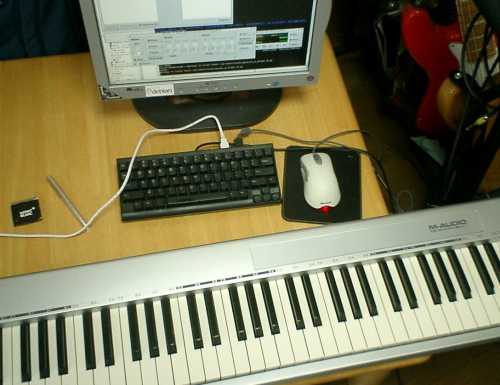
\includegraphics[width=0.8\hsize]{image200611/keystation.jpg}
\end{frame}

\begin{frame}
 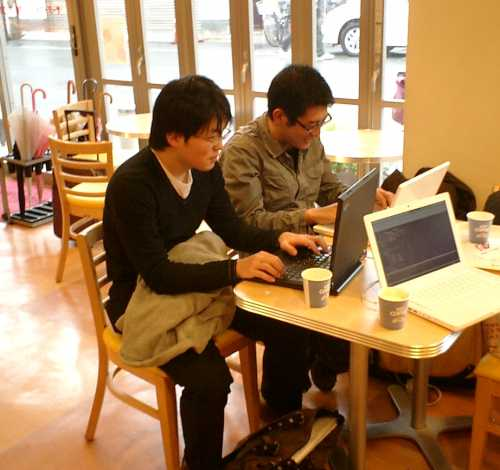
\includegraphics[width=0.8\hsize]{image200611/hack.jpg}
\end{frame}

\begin{frame}{上川}
今日の私の興味は、Debian 勉強会を関西で開催できるのか、どういう人がいる
のか、ということを確認することです。Debianについて活発に関西でもイベント
など開催されるとよいなぁ、と希望しています。
\end{frame}

\begin{frame}{浜辺さん}
課題未定出
\end{frame}

\begin{frame}{さとうさん}
課題未定出
\end{frame}

\section{sid とはなにものか}

\begin{frame}
\begin{center}
{\Huge sid とはなにものか}
\end{center}
\end{frame}

\begin{frame}{sid とはなにものか}

\includegraphics[width=0.8\hsize]{image200611/releases.png}
\begin{itemize}
 \item sid -- 別名 unstable 
 \item 毎日4AMに新しいバージョンがリリース
 \item 開発者のアップロードしたパッケージが入ってくる
 \item 最新版を利用できる環境
\end{itemize}
\end{frame}

\begin{frame}{インストール方法}
\begin{minipage}[t]{0.5\hsize}
  \begin{itemize}
  \item 安定版をインストールしてから sid にアップグレード
  \item chroot 内部に sid を飼う
 \end{itemize}
\end{minipage}
\begin{minipage}[t]{0.4\hsize}
 \begin{itemize}
  \item debootstrap
  \item cdebootstrap
  \item ツールの活用: pbuilder, dchroot など
 \end{itemize}
\end{minipage}

\vfill{}
chroot でメンテナンスして試験して、リスクを回避を推奨
\end{frame}

\begin{frame}{魅力}
 \begin{itemize}[<+->]
  \item 常にあらゆる最新版が利用できる
  \item 開発が起きている場
  \item オープンソースの世界の動きを肌で感じたいというのであれば、お薦め
  \item もし最新版のパッケージがそこにないなら、それを追加できるのは、あなた
 \end{itemize}
\end{frame}

\begin{frame}[containsverbatim]{情報源}
\begin{itemize}
 \item IRC: \verb!#debian-devel! 
 \item ML: \url{debian-devel@lists.debian.org}
 \item apt-listchanges
 \item apt-listbugs
\end{itemize}
\end{frame}

\section{bugreport 論}

\begin{frame}
\begin{center}
{\Huge bugreport 論}
\end{center}
\end{frame}

\begin{frame}{Debian BTS の特徴}
\begin{itemize}
 \item ウェブベースの表示インタフェース
 \item メールベースの変更インタフェース
 \item パッケージ単位でのバグ管理
 \item 安定性
 \item 公開
 \item バグの深刻さによる分類
\end{itemize}
\end{frame}

\begin{frame}{使われ方}

 深刻なバグ(RCバグ)

\begin{itemize}
 \item リリース不可判定
 \item ユーザのインストールの判断基準
\end{itemize}
\end{frame}

\begin{frame}{サーバのファイル構造}
\begin{minipage}{0.5\hsize}
  \begin{itemize}
 \item /org/bugs.debian.org/spool
       \begin{itemize}
	\item incoming/
	\item db-h/
	\item archive/
	\item index.db -- index.db.realtimeへのシンボリックリンク
	\item index.archive -- index.archive.realtimeへのシンボリックリンク
	\item nextnumber
       \end{itemize}
 \end{itemize}
\end{minipage}
\begin{minipage}{0.45\hsize}
 \includegraphics[width=0.9\hsize]{image200611/mirror.eps}\\
\hfill{}(推定)
\end{minipage}
\end{frame}

\begin{frame}[containsverbatim]{SOAP フロントエンド}
\begin{minipage}[b]{0.35\hsize}
 \includegraphics[width=0.7\hsize]{image200611/bugstruct.eps}
\end{minipage}
\begin{minipage}[b]{0.6\hsize}
  \begin{itemize}
  \item URL: \url{http://bugs.donarmstrong.com/cgi-bin/soap.cgi} 
  \item NS: \url{Debbugs/SOAP/Status}
  \item 提供されている関数: \verb!get_status(バグ番号)!
 \end{itemize}
\end{minipage}
\end{frame}

\begin{frame}[containsverbatim]{SOAP データ}
\begin{minipage}[t]{0.4\hsize}
  \begin{verbatim}
<item>326008</item>
<item>381350</item>
<item>389681</item>
<item>323626</item>
<item>334697</item>
 \end{verbatim}
\hfill{}
\includegraphics[width=0.4\hsize]{image200611/arrow.png}
\end{minipage}
\begin{minipage}[t]{0.5\hsize}
\begin{verbatim}
<?xml version="1.0" encoding="UTF-8"?><SOAP-ENV:Envelope
xmlns:apachens="http://xml.apache.org/xml-soap"
xmlns:SOAP-ENV="http://schemas.xmlsoap.org/soap/envelope/"
xmlns:xsi="http://www.w3.org/2001/XMLSchema-instance"
xmlns:SOAP-ENC="http://schemas.xmlsoap.org/soap/encoding/"
xmlns:xsd="http://www.w3.org/2001/XMLSchema"
SOAP-ENV:encodingStyle="http://schemas.xmlsoap.org/soap/encoding/"><SOAP-ENV:Body><namesp1:get_statusResponse
xmlns:namesp1="Debbugs/SOAP/Status"><s-gensym3
xsi:type="apachens:Map"><item><key
xsi:type="xsd:int">323626</key><value><found_versions
xsi:type="SOAP-ENC:Array" SOAP-ENC:arrayType="xsd:string[2]"><item
xsi:type="xsd:string">apt-listbugs/0.0.48</item><item
xsi:type="xsd:string">apt-listbugs/0.0.49</item></found_versions><done
xsi:type="xsd:string">Junichi Uekawa
&lt;dancer@debian.org></done><blocks xsi:type="xsd:string"/><date
xsi:type="xsd:int">1124298181</date><fixed
xsi:type="apachens:Map"><item><key
xsi:type="xsd:string">apt-listbugs/0.0.56</key><value
xsi:nil="true"/></item></fixed><fixed_versions xsi:type="SOAP-ENC:Array"
SOAP-ENC:arrayType="xsd:string[1]"><item
xsi:type="xsd:string">apt-listbugs/0.0.56</item></fixed_versions><mergedwith
xsi:type="xsd:string"/><found xsi:type="apachens:Map"><item><key
xsi:type="xsd:string">apt-listbugs/0.0.49</key><value
xsi:nil="true"/></item><item><key
xsi:type="xsd:string">apt-listbugs/0.0.48</key><value
xsi:nil="true"/></item></found><blockedby
xsi:type="xsd:string"/><keywords xsi:type="xsd:string"/><msgid
xsi:type="xsd:string">&lt;87wtmkld85.fsf@alhambra.kuesterei.ch></msgid><id
xsi:type="xsd:int">323626</id><forwarded
xsi:type="xsd:string"/><severity
xsi:type="xsd:string">serious</severity><owner
xsi:type="xsd:string">Nigel Jones &lt;nigel@nigelj.com></owner><subject
\end{verbatim}
\end{minipage}
\end{frame}

\begin{frame}{文化}
\begin{itemize}
 \item バグレポート修正
 \item 担当メンテナに報告、修正できないものは蓄積
 \item BSP 祭
\end{itemize}
\end{frame}

\begin{frame}{Debian JP Bug Squash Party on IRC}
 \begin{minipage}[t]{0.5\hsize}
  \begin{itemize}
   \item 2006年11月23日 10:00-15:00
   \item IRC チャンネル: osdn.debian.or.jp:debian-bsp? (iso-2022-jp) 
   \item 詳細は debian-devel@debian.or.jp, debian-users@debian.or.jp にアナウン
	 ス予定
  \end{itemize}
 \end{minipage}
 \begin{minipage}[t]{0.4\hsize}
 \end{minipage}
\end{frame}

\section{今後の予定}
\begin{frame}{今後の予定}
\begin{itemize}
 \item 2006/12/16 一年のしめくくりの会議、杉並区荻窪
\end{itemize}

 参加おまちしております
\end{frame}

\end{document}
